\documentclass{mprop}

% alternative font if you prefer
\usepackage{palatino}

% for alternative page numbering use the following package
% and see documentation for commands
%\usepackage{fancyheadings}
\usepackage{csquotes}


% other potentially useful packages
%\uspackage{amssymb,amsmath}
%\usepackage{url}
%\usepackage{fancyvrb}
%\usepackage[final]{pdfpages}

% Packages for image layouts
\usepackage{graphicx}
\usepackage{float}

\newcommand{\safealpha}{\(\alpha\)}

%% CUSTOM for todos taken from http://tex.stackexchange.com/questions/9796/how-to-add-todo-notes#9797
\usepackage[colorinlistoftodos,prependcaption,textsize=tiny,disable]{todonotes}
\newcommand{\timnote}[1]{\todo[linecolor=blue,backgroundcolor=blue!25,bordercolor=blue]{#1}}

\usepackage{enumitem}

\usepackage{cleveref}
\crefname{chapter}{\S}{\S\S}
\crefname{section}{\S}{\S\S}
\setcounter{secnumdepth}{3}
\crefname{table}{table}{tables}
\Crefname{table}{Table}{Tables}
\crefname{figure}{figure}{figures}
\Crefname{figure}{Figure}{Figures}
\crefname{appendix}{appendix}{appendices}
\Crefname{appendix}{Appendix}{Appendices}

\usepackage{float}

% \usepackage[round]{natbib}
\usepackage[style=authoryear,natbib=true,backend=bibtex]{biblatex}
\bibliography{biblio}


\begin{document}

\title{Investigating Computational Responsibility}
\author{William Wallis}
\matricnum{2025138}

\maketitle

\begin{abstract}
    Currently, models are produced for responsibility modelling which have their roots in logic. These models, while sophisticated, suffer from a lack of pragmatism: for guiding agent behaviour in sociotechnical simulations, logical models are not always ideal. In the similar field of trust modelling, algorithmic models which emulate social behaviour produce useful results while being easier to understand, implement, and reason about. In this paper\todo{paper? report? project?}, a proof-of-concept responsibility modelling platform adopting the algorithmic formalism style employed by trust modelling is produced, and its utility evaluated.
\end{abstract}

\section{Introduction}
A growing area of research lies in the formalism of human traits into computational representations. These algorithms make computers more human-like; for that reason, they are referred to here as ``Anthropomorphic Algorithms''\todo{improve the introduction of the Anthropomorphic Algorithms term}. A similar term, ``human-like computing'', has also risen in popularity lately. Human-like computing does not strictly focus on the implementation of formalisms of human traits, however, which is the area of interest for this report.\par

This implementation interest, realised in the study of anthropomorphic algorithms, presents an interesting sociotechnical problem. They present an opportunity to alter the behaviour of actors in a sociotechnical system, and to do so in a way that is easy to reason about. This alternation of behaviour is done by the algorithmic implementation of a \emph{formalism}. Formalisms present a concrete definition --- by process, mathematical definition or semantic description --- which can be used to construct an anthropomorphic algorithm. These formalisms tend to attempt to model in one of two ways:

\begin{enumerate}
    \item Modelling the trait as a useful metaphor\\
    These models tend to be inaccurate with regards the social science surrounding the trait that they model. However, they make a trade-off between this accuracy and the model's utility. For example, the notion of trust as a metaphor for a type of behaviour might be useful in information security research, but what matters in the formalisms implemented for this research is the formalism's utility in information security --- \emph{not} whether the formalism accurately represents human trust.
    \item Modelling social science directly\\
    These models attempt to accurately model the traits they concern. This can be useful for fields such as sociotechnical modelling, as well as social sciences research. There are also interesting applications for these models in interaction study: making interfaces interact with users in a human-like way, and representing the states of these traits to the users, are valuable research areas which are more applicable to these type-2 formalisms than to type-1 formalisms.
\end{enumerate}

In reality, most formalisms and their implementations lie somewhere on the spectrum that these two types define.\par

Current research focus has shifted slightly to consider the possibility of ``computational responsibility''; logical models of responsibility have been created previously. These models frequently regard responsibility as an ethical issue to model --- however, traits such as trust have been formalised for applications in fields such as information security. Along similar notions, responsibility might be formalised for the purpose of directing sociotechnical agent behaviour: this would allow the discharge of more important tasks earlier in the agent's timeline. Such a model of responsibility does not yet exist in algorithmic form. This report will present one such formalism of responsibility, complete with an algorithmic implementation, which is used to direct agent behaviour, as well as to improve agent behaviour over time by means of improving the agent's perception of responsibility.\par

The second section of this report focuses on exploring the problem domain, and making concrete the research questions which this report will address. The third section follows this with a review of important literature from areas in anthropomorphic algorithms and sociotechnical systems research which might inform this proof-of-concept formalism. A fourth section then explores design philosophies which can be adopted from lessons learned in the background survey, and this is then followed by a specification of the formalism's constituent parts. An evaluation of the formalism outlined follows in the fifth section, and work building on the formalism presented --- and the results of the evaluation --- are presented in the sixth section. The report concludes with a discussion on what has been presented, and the work which this exploration into a new anthropic trait turned anthropomorphic makes possible.\par

\section{Statement of Problem}
Computational formalisms of human traits are a growing field of research, with applications in lots of different areas. A problem with these anthropomorphic algorithms is that there is limited breadth to the scope of existing research in the field (as is demonstrated during the background survey in \cref{sec:related_work}). The metaphor of the human trait in these algorithms remains largely unexplored.\par

Breadth in the application of the metaphor is important, however. The importance stems from the utility in the human metaphor when designing systems:

\begin{itemize}
  \item Human-Computer Interaction can make use of behavioural metaphors to relay complicated internal states to a user. Storer et al.~\cite{storer_mobile_behaviour_poster} demonstrated methods by which a mobile device might dissuade certain user actions by expressing its ``discomfort'' or lack of ``trust'' in its interaction design.
  \item Information Security can make use of behavioural metaphors in order to increase difficulty of access when negative system states are encountered. A system might allow access on a graded scale, dependant on internal states of trust, comfort, and confidence.
  \item Theoretical advancements in smart city technology\cite{wallis_talk_about_x_talk} might increase a city's resilience by integrating notions of responsibility into public services and the environment on a community scale.\par
\end{itemize}

While similar results can often be achieved using regular techniques, the human metaphor allows for a better communication between a human user and complicated system states. All of the above examples center around this notion; however, the applications extend beyond Human-Computer Interaction research.\par

The lack of application of the human metaphor is a complicated mosaic of related factors. For example, research into anthropomorphic algorithms holds particular challenges, as a result of its strongly interdisciplinary nature: it requires a research team to understand the nuances of sciences as well as social sciences, and sometimes even humanities. Not only does the research team require the ability to understand these nuances, but the research must take into account their different natures. This often causes divergence in the philosophies of sociotechnical research. Some researchers view sociotechnical systems from the perspective of largely human-based systems with abstract, social behaviour. Others see sociotechnical systems as a combination of dynamic, mathematical processes which produce more technical emergent phenomena. This hints at a third complicating factor, (the second being a lack of convergence in research focus): a lack of a consistent modelling paradigm. Some research focuses largely on actor interaction-style modelling techniques~\cite{baxter2011socio}, while others rely on purely graphical modelling~\cite{ObashiMethodology}, or on mathematical modelling techniques~\cite{vespignani2012modelling}. \par

These issues together pose an issue for research in anthropomorphic algorithms: a formalism of a human-like trait is only useful to certain researchers, for certain types of models, with certain sociotechnical philosophies. Their lack of broad application is therefore unsurprising; these factors compound to produce yet another, which is that the breadth of traits formalised and researched is very small. The largest degree of research is easily conducted in the field of Trust; other traits, such as Comfort, have recently been attempted also~\cite{marsh2011defining}.\par

Recently, some interest has been shown in research pertaining to modelling and formalising \emph{responsibility}. Logical models of social trust exist which could be turned into a proof-of-concept formalism of responsibility with only a small addition: adding an obliging term in a similar way to the Deontic Logic's system for obliging\cite{deontic-logic}, allowing an agent to effectively delegate a task to another which is deemed responsible in discharging responsibilities --- the agent selected being known to be trusted already, by C\&F's already established work. The scheduling of tasks based on trust is a simple extension of existing models, or an application of existing models.\par

A model of responsibility might be more than simple task allocation, however. Some logical models of responsibility attempt to model ethically responsible decisions~\cite{berreby2015modelling}. Deontic logic's obliging term was in itself an attempt to create a logic which was suitable for the calculation of whether an agent was obliged to ensure certain goals, or perform certain tasks. Another angle might be to perceive a model of responsibility as something which might allow a responsible sociotechnical agent to choose responsibilities to discharge, rather than blindly executing tasks they are provided with in a trust-oriented model which simply delegates tasks.\par

The latter has a number of potential applications. One such possibility would be to implement agent awareness of remote task execution via RPC\@. Should an agent on a network be given a procedure to execute which is perceived through a responsibility formalism to be unusual, the procedure may not be executed, or may be rejected upon receipt by the responsible agent. Similar applications have proven effective in trust literature, particularly the Eigentrust algorithm~\cite{eigentrust}~, where information security is enhanced by inferring agent trustworthiness.\par

In a realistic sociotechnical system, an agent's behaviour is often informed via a feedback loop. It is important, therefore, to allow an agent to learn better ``responsible'' behaviour over time, through an analysis of its sociotechnical environment and other factors. In acknowledging that anthropic traits are most useful when they account for both introspection --- so as to direct an agent's own behaviour based on the formalised trait --- and extrospection --- so as to judge and learn from that trait in other agents.\par

To achieve these goals, two research questions were formulated:

\begin{enumerate}\label{RQ}
    \item How can a computational formalism of responsibility direct the decisions made by an intelligent agent?
    \item How can an intelligent agent assume the consequences of actions it makes, the decisions other agents make, and its general environment, so as to direct its interpretation of responsibility?
\end{enumerate}\par

Answering these questions requires the construction of a proof-of-concept formalism of responsibility which is suitable for directing agent behaviour in an algorithmic manner, as opposed to existing logical methods.

\section{Related Work}\label{sec:related_work}
A broad range of literature must be reviewed to properly understand the research at hand, due to the problem's broad nature. Particularly, this paper\todo{paper? report? project?} will focus on three areas: popular algorithmic trust models; broader sociotechnical systems research; and relevant philosophical literature.\par

\subsection{Trust Modelling}
Ordinarily, when constructing a new anthropomorphic algorithm, one would draw on literature regarding other anthropomorphic algorithms which formalise the trait being modelled. However, no such formalism exists for responsibility modelling; therefore, insights from early trust modelling may provide useful information on how to proceed, given that responsibility formalism now is in a similar stage to early trust formalism. Trust is particularly appropriate as a comparative trait to responsibility, as the two traits have many similarities (as investigated earlier).\par

\subsubsection{Marsh}
The seminal anthropomorphic algorithm for trust is found in Marsh's 1994 formalism\cite{Marsh1994FormalisingConcept}. In this paper, a formalism is described which has a number of useful qualities: it is modelled on a per-agent basis as opposed to calculating trust across a group of agents, has foundations in social sciences, and is largely algebraic, staying clear of modelling via logic.

Of particular interest is Marsh's separation of three different degrees of granularity in trust judgement. Marsh identifies that human agents have a basic degree or weighting which applies to their trust --- it would not be uncommon to assert that ``person X is very \emph{trusting}''. This is, however, distinctly different to an assertion that ``person X is trusting, but \emph{doesn't trust person Y}'' --- that is, a person's basic level of trust is distinctly different from a person's more directed degree of trust toward another agent in particular. Marsh calls this ``General Trust'', differentiating it from the earlier ``Basic Trust''. A final distinction, ``Specific Trust'', identifies an agent's degree of trust in another with regards a specific task (which could be considered ``person X's degree of trust in person Y \emph{in doing task \(\alpha\)}).\par

These separations are useful in a few key ways. One is that it identifies some of the key parameters in the model of trust: at the very least, Marsh's formalism of trust requires an agent, two agents, or two agents and a task or action in order to calculate a degree of trust. This is useful when generating a model of responsibility, as trust and responsibility share some common features: like trust, responsibility usually concerns two agents, and a task that one agent is responsible for. Unlike trust, responsibility modelling contains hierarchies: one agent might be considered the authoritative figure, which \emph{delegates} a task to another. For the purposes of this paper\todo{paper? report? dissertation? project?}~, the latter agent will be referred to as a ``delegee''. The similarities in the parameters of the formalism affirm the notion that responsibility and trust are similar in concept, and also serve as a starting point for imagining what an algorithmic formalism of responsibility might be like.\par

Another useful insight from these separations would be that, when considering responsibility, judging how responsible an agent is can be done from the same three vantage points. Basic responsibility would colloquially be ``benefit of the doubt'', general responsibility would be how responsible an agent in all modelled capacities, and specific responsibility would be another agent's calculated responsibility with regards some task, resource, or other modelled subject of responsibility). Not only does this also affirm trust and responsibility's similarities, but it helps in providing further structure to the new formalism.\par

A final important property of Marsh's formalism is its graded nature. This model does not produce a boolean indicator of whether to trust or not; rather, it opts to calculate a number between 0 and 1 of the \emph{degree} of trust one agent ought to have in another. This feature allows for as granular a model of trust as any given application requires, and allows for more nuanced comparison between agents.\par

\todo{Write more of this? Maybe less on the separations, and more on its social science background or lack of logical foundation?}

\subsubsection{Castelfranchi \& Falcone}
Another useful formalism of trust to consider comes from Castelfranchi \& Falcone~\cite{CastelfranchiSocialApproach} (often referred to as ``C\&F theory''). While this formalism has logical foundations, its large popularity makes it an interesting comparison to Marsh's formalism.\par

In contrast to Marsh's formalism, C\&F is graded only in more complex forms. At its root, C\&F is a logical formalism built on boolean calculations of goal and belief state satisfaction. However, C\&F also segregate different aspects of trust in their formalism: different elements of the basic formalism represent competence, disposition, and dependence. They define competence as one agent's belief and will that another agent can successfully achieve a goal by a certain action, disposition as the belief and will that the other agent is willing to perform an action to achieve a goal, and dependence as the effective delegation of a task for the purpose of achieving a goal (expressed via logical statements).\par

Curiously, the C\&F model of trust contains all of the same parameters as Marsh's, plus a fourth: the goal to be achieved by an action. One may take the position that a goal is also important in modelling responsibility --- but it is not immediately apparent that it is necessary to include it. Therefore, C\&F uncovers the need when building a formalism of a trait to make choices as to the formalism's philosophy regarding the trait.\par

In particular, two philosophical differences between Marsh's model and that of C\&F are immediately apparent: where Marsh separates his calculation of trust into a basic/general/specific granularity, C\&F separate trust's different constituent parts, each of which must be satisfied for trust to be present. Another philosophical difference between the two is the assertion as to whether the goal of an action factors into one's trust. These philosophical decisions can make concrete, important differences to a formalism's constitution --- which is plain to see when considering that even the parameters of the model differ, something fundamental to the formalism's definition of trust. Therefore, these choices as to the approach to responsibility are important to note in the formalism produced during this report\todo{report? paper? Dissertation?}.\par

\subsubsection{Eigentrust}
Eigentrust\cite{eigentrust} is a formalism which takes a notably different approach to Marsh and C\&F's formalisms: rather than attempting to model human trust accurately, it models trust as a metaphor for the truly desired behaviour.\par

Calculations of trust in Eigentrust have their foundations in eBay's model for reputation: star ratings based on a summation of satisfaction scores. In particular: \[s(i,j) = sat(i,j) - unsat(i,j)\]~\ldots{}where \(sat\) is the number of satisfactory interactions between two agents and \(unsat\) the unsatisfactory ones, represents a ``local trust value'' that an agent \(i\) has in another agent \(j\). Through some linear algebra, these local trust values are accumulated and gradually turned into a global score of responsibility, accounting for all agents' opinions of each other. This global score could also be considered to be an agent's \emph{reputation} --- in this way, Eigentrust generalises trust as a certain application of a reputation formalism, and bootstraps its own formalism on another trait.\par

While Eigentrust has proven particularly effective in its intended domain, it is a formalism designed expressly for the purposes of network and information security. Eigentrust achieves this by a number of philosophical differences to Marsh and C\&F's respective formalisms:

\begin{itemize}
    \item Eigentrust operates in a distributed way. Unlike the local scoring system employed by Marsh and C\&F's formalisms, Eigentrust has all agents report their local trust scores, so as to create a distributed ledger of more general trust scores.
    \item Eigentrust does not model trust directly, nor does it claim to model it accurately --- unlike C\&F's formalism, which is strictly intended as a model of human behaviour, and Marsh's, which simulates it, Eigentrust uses ``trust'' as a description of an agent's behaviour.
    \item Eigentrust is not concerned with the cause of satisfactory or unsatisfactory interactions; it focuses entirely on accumulated positive/negative scores. In this way, Eigentrust somewhat models Marsh's ``general trust'', but makes no assertions as to trust's composition or how to reason about it.
\end{itemize}

In these respects, Eigentrust represents an interesting alternative end of the spectrum between anthropomorphic algorithms which treat their trait as a metaphor, or as a social behaviour to accurately simulate. While Eigentrust does not represent a very useful foundation for our responsibility formalism, it does highlight two things:

\begin{enumerate}
    \item The responsibility formalism required to test the research questions should be more similar to Marsh and C\&F's formalisms than Eigentrust: there is no specific use case to design for, so designing with a trait as a metaphor would not be appropriate.
    \item Should it be necessary, a trait's formalism could be bootstrapped using a pre-existing formalism of another trait. Whether this is a suitable way to answer the research questions above is harder to address; the possibility should therefore be considered.
\end{enumerate}

\subsubsection{FIRE}
FIRE\cite{huynh2004fire} is another trust modelling system which provides a focus on being able to judge trust using information from many different sources. For example, it treats direct experience  information in a different way to information collected by third parties. It is also a model which considers multiple different traits: it incorporates reputation information into its judgement of trust. In part, FIRE is able to do this because it segregates different information sources into different measurements, which are tabulated into a score after their measurement.\par

FIRE's inclusion of information from multiple sources paints other trust formalisms in a slightly different light. However, this feature is not necessary for all trust scenarios: the decision to trust (or not trust) is made with different amounts of information for agents in different simulations. One can imagine a two-agent simulation, where information about each agent's interactions would be assessed by exactly one source --- the other agent, which judges the former's reliability. It is plain to see that FIRE is designed to be a formalism treating traits as a metaphor, similarly to Eigentrust.\par

This philosophical decision makes FIRE an unlikely candidate as a foundation of a responsibility formalism, as its specific application area --- sociotechnical models with multiple types of information to consider --- is more complex than is necessary for a proof-of-concept responsibility formalism, and would be more complicated than the research questions posed require. However, the philosophical choice it raises regarding different types of information, and the nature of the information which is being reviewed when calculating the responsibility score, is an important one.\par

% TODO: should this be 'sociotechnical systems', 'Ian Sommerville', or 'Responsibility Modelling'? What's a good title? Is there anything other than Sommerville to go in here?
\subsection{Sociotechnical Systems}
While these anthropomorphic algorithms are useful to consider in isolation, their application within the realm of sociotechnical systems is important to their design. Moreover, the nature of responsibilities is touched within the broader sociotechnical systems area of responsibility modelling --- research on the delegation and discharge of responsibilities, and how to reason about them.\par

\subsubsection{Ian Sommerville}
\todo{What more can we say about Sommerville's contributions? At the moment we only cover consequential and causal responsibilities.}
Ian Sommerville was a prolific writer in the field of sociotechnical systems, who was responsible for much of the current literature on responsibility modelling\cite{sommerville_graphical_responsibility,sommerville_dependable_systems_chap_8,sommerville_dependable_systems_chapter_9}.\todo{What other references can go here?} Sommerville's responsibility modelling systems often happened to be graphical\cite{sommerville_graphical_responsibility}, a paradigm for computational responsibility which may prove hard to convert to an anthropomorphic algorithm. This is because graphical representations of system states do not naturally present themselves as a numerically analysable format for information --- rather, graphical presentations are useful for exposing sociotechnical system state. This feature of sociotechnical modelling, and particularly responsibility modelling, is useful for risk and impact analysis\cite{ObashiMethodology}.\par

Sommerville's writing, however, presents a wealth of interesting insights which may be useful in understanding the context of the anthropomorphic algorithm, and understanding some possible choices as to the formalism's philosophy.\par

In particular, Sommerville notes an interesting distinction as to two different sorts of responsibilities: ``consequential'' and ``causal'' responsibilities. They can be thought of as the difference between a responsibility for a current state --- the result of a previously discharged responsibility --- and responsibility for producing a future state --- a change to a current state that an agent is responsible for bringing about in the future.\par

Sommerville's separation clarifies a potential avenue by which one might create a computational responsibility formalism. Namely, an agent's degree of responsibility might be associated with the state changes they have brought about in the past, and perhaps a prediction of the chance that an agent would discharge a causal responsibility successfully at some future time. This approach, verified by its appearance in existing sociotechnical systems literature, may be appropriate for creating a computational responsibility formalism, though its foundations exist in a less useful graphical representation approach.\par

\subsubsection{Timothy Storer \& Russell Lock}
\todo{tim or timothy?}
While describing a graphical responsibility modelling format for the InDeED project --- notably lead by Ian Sommerville --- Storer and Lock provide some useful foundations for other models of responsibility in a technological report on modelling responsibility\cite{storer2008modelling}.\par

Most interestingly, Storer and Lock provide a useful definition of a responsibility:

\begin{quotation}
    A duty, held by some agent, to achieve, maintain or avoid some given state, subject to conformance with organisational, social and cultural norms.\cite{storer2008modelling}\par
    
    \ldots{}\par
    
    Responsibilities are the duties to be discharged by agents as described\ldots{}
\end{quotation}

Numerous things in this definition are useful. Similarly to the work done by Mash and C\&F, the definition provides an insight into some possible fundamental parameters of a responsibility:

\begin{description}
    \item [A duty: ] responsibilities can be considered as some action an agent is \emph{obliged} to conduct.
    \item [achieve\ldots{}some given state: ] the obligation which a duty is defined by can be described as a change of \emph{state}. Storer and Lock note that this state change can have different modes: it can be achieved, but also maintained or avoided. It is worth noting that this very general description of responsibility indicates that the graphical formalism designed for the InDeED project was somewhat socially accurate.
    \item [comformance with\ldots{}norms: ] agents can be delegated responsibilities in most useful formalisms of responsibility --- Storer and Lock note that these responsibilities must not conflict with norms that an agent holds.
\end{description}

Unlike Marsh or C\&F's more mathematical definitions of trust, this semantic definition lends itself nicely to conversion to some responsibility model; partly because it already summarises the responsibility trait, but also because it describes an intuitive social definition of responsibility while remaining very simple. Therefore, a responsibility formalism which somehow extended this model, while retaining the power of the anthropomorphic algorithms described earlier would provide a very useful starting point for the desired responsibility formalism.\par

Another useful definition from Storer and Lock's report presents itself when discussing the structure of a responsibility in their model:

\begin{quotation}
    Responsibilities may be composed of other responsibilities.
\end{quotation}

This composibility is an interesting property, which may also imply that some responsibilities can be broken down into a form of sub-responsibility. This property would be useful to remember when modelling responsibilities in the desired formalism. It also implies that there may be a sort of ``atomic'' responsibility, that more complicated responsibilities are composed of.

\subsection{Philosophical Literature}  % The nature of responsibility, and the validity of modelling anthropic traits in a machine.
As responsibility is a social trait, and previous literature has indicated that it may be most appropriate to model it as such, input from literature in the humanities may shed light on how to consider and approach responsibility as a trait accurately. As time allowed for this report was somewhat limited, a more complicated sociologically/psychologically accurate model was not attempted. The decision was made to instead create a proof-of-concept model which encapsulated much of the existing sociotechnical systems literature, and verifying it using philosophical literature on the subject.

\subsubsection{Thomas Scanlon}  % A philosophical perspective which converges on Sommerville's ideas in Dependable Systems
Thomas Scanlon --- a philosopher who specialises in Analytic Philosophy --- writes on responsibility in the essay ``Justice, Responsibility, and the Demands of Equality'', defining terms which bear striking resemblance to Sommerville's ``Consequential'' and ``Causal'' responsibilities.\par

One term --- ``attributive'' responsibility --- is defined by Scanlon as being:

\begin{quotation}
    What a person sees as a reason for acting, thinking, or feeling a certain way\cite{scanlon2006justice}
\end{quotation}

This might be generalised as being the responsibility for future and current action, as attributive responsibilities would clearly be the influencing responsibility of a future action. If future actions discharge the responsibilities an agent possesses at a given time, then Scanlon's ``attributive'' responsibilities in effect mirror Sommerville's ``causal'' responsibilities.\par

Scanlon goes on to define a second term, ``substantive'' responsibility, which can be described loosely as a responsibility for an action fixed in the past. Given the sociotechnical perspective of responsibility being a change of sociotechnical state, Scanlon's ``substantive'' responsibilities also seem to mirror a term of Sommerville's, namely his ``consequential'' responsibilities.\par

Given the convergence of this perspective on responsibility --- that is, the separation of past state change and anticipated future state change --- Scanlon's writing seems to affirm Sommerville's own construction of types of responsibility --- though clarity on how this distinction is useful is found in work from another philosopher, P.F. Strawson.\todo{I feel like this segue is pretty poor! How can I improve this?}

\subsubsection{P.F. Strawson}  % The nature of responsibility
P.F. Strawson is a philosopher with work on philosophy of language and of mind --- one particular essay, ``On Freedom and Resentment''\cite{strawson}, presents an argument that determinism shouldn't affect how we perceive human factors such as responsibility or trust.\par

Strawson argues that these concepts are fundamentally relational, rather than having any inherent definition. The conclusion of this is that trust, responsibility, and other human traits have subjective properties and cannot be calculated outside of the perspective of an agent. This hints at a choice as to the desired formalism's philosophy: unlike a formalism such as Eigentrust, where components of trust scores are calculated independently of any one agent's perspective, the required responsibility scoring system must utilise a subjective perspective for \emph{all} calculations. Strawson's argument applies to sociotechnical systems, as it does not apply to any specific trait or type of person; therefore, both social and technological actors in a sociotechnical system might be the targets of a trait designed with Strawson's work in mind.\par

Strawson also produces a fairly rigorous analysis of how ordinarily variable human traits can be formalised:

\begin{quotation}
    Indignation, disapprobation, like resentment, tend to inhibit or at least to limit our goodwill towards the object of these attitudes, tend to promote an at least partial and temporary withdrawal of goodwill; they do so in proportion as they are strong; and their strength is in general proportioned to what is felt to be the magnitude of the injury and to the degree to which the agents will be identified with, or indifferent to, it.\cite{strawson}
\end{quotation}

Strawson here identifies a similar property of human traits to Marsh: when an agent acts, the magnitude of the judgement of a trait with respect to the act is proportional to the magnitude of its effect on an overall judgement of the trait. That is to say, if an action has a given importance, the magnitude of that importance should carry through to judgements that the action impacts. This, combined with the subjectivity implied by the earlier point made by Strawson, implies that importance might be interpreted subjectively.\par

The introduction of a parameter of importance associated with a responsibility score allows the magnitude of importance of an act to be quantified and tracked in consequential or substantive responsibilities, adhering to Strawson's second point. Should some mechanism for interpretation be provided by the formalism, a subjective factor is introduced, satisfying Strawson's first point. This also hints at how an agent might judge the degree of responsibleness of itself or another agent, helping to answer the second research question; Strawson's argument here is therefore useful in the construction of the desired computational responsibility formalism.\par

\subsubsection{Sloman}  % The space of artificial minds, and a brief note on the philosophical value of this formalism (optional!)



\section{A Formalism of Responsibility}

\subsection{Design Decisions and Philosophy}

As was discussed through the background survey, many different philosophical decisions are made explicitly or implicitly during the creation of an anthropic formalism. In order to be certain of the finer details of the model created, then, it is important to clarify some of the choices made.\par

% Decision to be socially accurate
%  - There's no specific application area, so we should focus on modelling responsibility as a general trait, rather than solving a specific problem. 
%  - The research questions are best answered by a non-application-oriented formalism, because they're describing aspects of a responsibility formalism, not a responsibility formalism in a certain setting!
%  - We're not trying to solve any issue perceived in other anthropomorphic algorithms, like FIRE does.
\subsubsection{Social Accuracy}
Firstly, the formalism created should be socially accurate. No specific application area presents itself for this formalism; rather, the work presented is intended as a proof-of-concept for anthropomorphic algorithms pertaining to responsibility. A formalism which used responsibility as a metaphor would be inappropriate, as no purpose for the metaphor readily presents itself. In addition, no specific issues with existing formalisms are intended to be solved by the formalism --- this is at odds with the background of a formalism such as FIRE, which was created specifically to solve the issues with existing anthropomorphic algorithms for trust. As current efforts in computational responsibility have their roots in logic, no anthropomorphic algorithm for responsibility exists to provide issues to solve. Therefore, the algorithm created should be a proof-of-concept with a focus on social accuracy.\par

% Decision to be decentralised --- no need to communicate judgement scores, agents calculate all on their own.
\subsubsection{Decentralised Information Exchange}
The formalism created should also allow for decentralised calculations of responsibility importances and judgements of responsibleness. Centralised calculations of these properties might be useful for specific application areas --- such as Eigentrust's focus on information security, where all agents communicate their states to all other agents so as to have all peers on the network as well-informed as possible. The desired responsibility formalism, however, should allow agents to operate individually, so as to create more socially accurate models (as not all information is guaranteed to be passed around a group of peers. One possible way to create a responsibility formalism with particularly well-informed peers would be to make use of recent work on computational gossip\cite{Boyd2006,Lavaei2012}: this would allow peers to communicate responsibility metrics in a socially accurate way. However, this is beyond the scope of this proof-of-concept project.\par

% Decision to judge responsibility based on the success/failure of an action to meet an action's requirements (in answer to the question FIRE raises, on what sort of information the formalism considers)
%  - Based on the literature describing consequential/causal responsibility.
%  - We calculate causal responsibilities based on the known consequential responsibilities.
\subsubsection{Information the Formalism Regards}
The FIRE algorithm raises a second question as to the desired formalism's philosophy: FIRE is designed to solve the issue of judging information differently depending on its origin. A decision as to the information sources the designed formalism should consider should be considered. As the formalism created is intended to be a relatively uncomplicated proof-of-concept, the fewest information sources required to allocate, accept, discharge and judge responsibility should be modelled in this first formalism.\par

Work by both Sommerville and Scanlon indicate that a suitable degree of information for the judgement of responsibleness for causal responsibilities would be the previously discharged consequential responsibilities. Therefore, the formalism's responsibility judgement should focus primarily on the information recorded regarding these past responsibility discharges, their associated changes to sociotechnical state, and the successes of those state changes.\par

Strawson's writing provides some more useful insights regarding information needed when selecting responsibilities to discharge, as well as judgement of past responsibilities: each responsibility should have associated with it an importance, so as to consider Strawson's ``magnitude of the injury'' (or, here, sociotechnical state change). Therefore, information which this formalism should consider consists of consequential responsibilities of an agent, and those responsibilities' relative importances.\par

% Decision not to care about act, but to describe outcome (effectively the goal)
\subsubsection{Responsibility Composition}
The content of a responsibility can be somewhat clarified at this point. In particular, C\&F's formalism of responsibility made clear that, in trust, the fundamental parameters they considered were a delegating agent and an agent subject to delegation, a desired action, and the goal the action ought to fulfil. Marsh, however, considered the action, but left his fundamental formalism devoid of a notion of goal.\par

In the desired responsibility formalism, nuances in the nature of a responsibility must be considered. Particularly, sociotechnical literature on a responsibility points to considering responsibilities as descriptions of state change, which ideally are composable. This state change could be considered the intended or required outcome of successfully discharging the responsibility --- however, it does not imply any information regarding the action which brings about this state change.\par

Therefore, a responsibility formalism's fundamental parameters would appear to be an authority agent and a delegee, subject to responsibility delegation from the authority agent, plus a composable model of state change describing the responsibility itself. In addition, the desired formalism for this project\todo{project? paper? report?} should include importance information as a fourth parameter, allowing for responsibility selection and responsibleness judgement as previously discussed.\par

% Decision to make the formalism subjective
%  - Different agents in the real world have different ``opinions'' about responsibility
%  - If the model is to be socially accurate to a degree, we should include a mechanism for different agents to see different responsibilities differently.
\subsubsection{Subjectivity}
The required formalism ought to allow for subjective, agent-based ``opinions'' regarding the importances of modelled responsibilities. As importance is to be directly measured in this formalism, a mechanism by which an agent might interpret the importance scores of responsibilities would allow for a subjective measurement of responsibility importance, allowing an agent to perceive its own model of the trait according to its ``opinions'' about responsibility. These might be considered its preferences for responsibility selection, which weight the importances in its accepted responsibilities. A specific example of an interpretation function is given in the specifics of the formalism designed below.

\subsubsection{Graded Responsibility Calculation}
A degree of responsibility should be calculable in a \emph{graded} form, rather than binary. In Trust models such as Eigentrust, or Marsh's formalism, degrees of trust are represented numerically so as to better delineate between different trust measurements. By contrast, other models --- particularly logical trust models --- represent degrees of trust in a binary format, such as C\&F's basic form does.\par

The feature of graded measurement is useful for a few reasons. The feature is principally useful for comparison between many different agents when judging lots of responsibilities --- task delegation amongst a pool of potential candidates being one scenario where this is useful. The feature therefore makes the formalism more pragmatic. Another benefit of a graded formalism is that it allows for a higher degree of social accuracy: human judgement of responsibility is much more nuanced than a simple boolean judgement. Finally, a graded formalism allows for a deeper exploration of its efficacy. In order to evaluate the formalism properly, comparisons between agents with a responsibility formalism directing their behaviour and others with no such direction should be modelled.\par

\subsection{Specific Formalism Details}
\todo{Is there a better title for this subsection? Supposed to be details of the actual formalism which was designed with these design philosophies in mind.}

Related research has helped to inform many design choices surrounding the formalism required to fulfil the research questions which this project\todo{project? paper? report? dissertation?} answers. As the necessary design decisions are now properly understood, a computational responsibility model which conforms to these design choices can be constructed.\par

The components of the formalism defined by this paper are Constraints, Obligations, Responsibilities, Importances, Agents, an Interpretation Function, and a mechanism for judging the responsibleness of any given agent.\par

\subsubsection{Constraints}  % Constraints are the "atomic responsibilities" defined earlier. It's the fudamental unit of state change that Storer describes earlier.
A responsibility, for the purposes of this model, will be considered a state change in a sociotechnical environment. This definition is insufficient for modelling a responsibility, however, as metadata such as delegee, authority, and importance should also be defined. In addition, it should be possible to compose these sociotechnical state changes.\par

To achieve this goal, Constraints are introduced. Constraints are descriptions of a sociotechnical state change. Storer \& Lock's idea of a composable responsibility form implies an atomic responsibility which cannot be \emph{decomposed} --- Constraints satisfy this atomic property.\par

The model also defines two types of constraints:

\begin{description}
    \item [ResourceDelta: ] a constraint which describes a set of changes to a number of variables (referred to here as a ``resource'') in the sociotechnical environment. The delta associated with the variable is described as a floating point number.
    \item [Deadline: ] the expected duration of the task. This constraint is special, because it is also provided with a clock for reference so as to calculate time relative to the constraint's reference frame --- clocks are provided by the Theatre modelling library\cite{theatre_code}. They are otherwise similar to a ResourceDelta.\todo{check that this citation has worked properly --- it's a reference to a Github repo...}
\end{description}

Using these two constraint types, changes to the sociotechnical environment are recorded as specifications for a responsibility discharge. It is imperative to note that the constraint creation does not include an importance, even though the design philosophy of the formalism is to give each responsibility a formalism. A Constraint is the atomic definition of a responsibility's effect; therefore, all constraints must eventually receive importance scores. An importance score cannot be provided upon the creation of a constraint, however, as the constraint simply describes a sociotechnical state change --- an importance score is a detail which only becomes necessary upon responsibility delegation, as different delegees may be required to meet the same state change specification with different importances. Constraints are therefore initialised without importance scores.\par

\subsubsection{Obligations}  % Sets of constraints. An obligation is a description of a responsibility's effect, but doesn't concern itself with metadata like the discharging agent.
Obligations are sets of Constraints --- they therefore allow Constraints to be composed together. Obligations may only concern themselves with a single Constraint, but defining a specific type which contains all Constraints a Responsibility is concerned with allows for a complete specification of that Responsibility's effect on the sociotechnical environment.\par

An Obligation therefore defines the complete sociotechnical effect which is defined by Storer \& Lock as a responsibility --- however, it concerns itself with no metadata as to the specific responsibility it serves as a specification of. Obligations might rather be considered a Responsibility which has not been delegated: details such as authority and delegee are not specified, but the sociotechnical definition of the responsibility is fulfilled. Additional information is supplied only when this Obligation is delegated.

\subsubsection{Responsibilities}  % An assigned obligation, with an authority and a delegee. Explain that importances are also introduced here, as the same obligation may be important to different delegees in different ways. Properly define the term "discharge"
The act of delegating necessarily defines certain details pertinent to a complete Responsibility. These details include the authority and delegee associated with the Responsibility --- this relational information is defined by the act of delegation.\par

Importance scores can also be introduced at this point, as the delegee is defined; therefore, information scores can also be assigned, as the only factor preventing information score allocation upon the initialisation of a Constraint is that the discharging agent --- the delegee --- was not defined. The importance scores are provided as floating points in the range \([0,1]\), and are provided as a list in the same order as the constraints provided to the Obligation.\par

A Responsibility is used by an agent in the sociotechnical system for selecting a next task --- to aid this, Responsibilities provide some convenience methods. In particular, Responsibilities allow for calculating specific details regarding the Obligation it is initialised with, such as the cumulative effect of the various Constraints it is defined by. In the implementation for testing this formalism, the effect of a Responsibility was contained in a ResponsibilityEffect object --- this allowed for providing further convenience methods, allowing one to get the total effect on one particular resource (from all contained ResourceDelta Constraints), or to disregard any particular resources which were effected when reasoning about the effect of a Responsibility.\par

\subsubsection{Agents}  % Briefly describe Theatre model for agents and their workflows. Define authorities and delegees.
An Agent consists of two important pieces of functionality:

\begin{itemize}
    \item Interaction with a sociotechnical modelling framework.
    \item Task selection and responsibleness judgement using the responsibility formalism.
\end{itemize}

Useful sociotechnical modelling frameworks for utilising the formalism are workflow modelling frameworks which maintain a consistent reference frame across all actors. Should the framework allow for online workflow modelling --- workflows where the next item in the workflow is not predetermined --- then a workflow can be constructed during the model. This permits a non-deterministic model execution, which is vital, as task selection according to the formalism is subjective.\par

Agents also contain their own sociotechnical state. This should contain all of the variables that a Obligation describes as being altered in some way. In addition, they are given a ``basic responsibility score'' --- this number, in the range \([0,1]\), represents a ``benefit of the doubt'' responsibility judgement for basic responsibility calculations. It is used in judgement of responsibility, which is described below.\par

To achieve subjectivity, agents are expected to contain interpretation coefficients; details regarding the interpretation coefficients are given in the Interpretation Function section\cref{subsec:interpretation_function}.\par

Agents should be defined with a set of responsibilities upon initialisation, which are referred to as notions. Notions represent responsibilities an agent may always discharge, such as an agent's option to idle away a clock tick without doing anything. Notions, unlike delegated responsibilities, are not removed from an agent's list of available responsibilities upon discharge. Notions are equivalent to the ``norms'' defined by Storer \& Lock\cite{storer2008modelling}.\par

Agents are complicated entities which implement the entire anthropomorphic algorithm described in this report\todo{report? paper? dissertation? project?} --- two particular elements of the Agent's implementation are Acts and the Interpretation Function, which are detailed below, in their own sections.

\subsubsection{Acts}
A workflow model is particularly useful for the construction of Acts.\par

An Act is supplied as a Higher Order function, paired with a ResponsibilityEffect, and are registered via a method on an agent. This is done so that the expected effect of the function on the sociotechnical model can be compared against responsibilities that an agent has. When discharging a responsibility, all Acts an agent has registered are compared by their effects against the expected effect of the responsibility discharge. If they match, the responsibility is discharged by executing the function associated with the Act. Upon act completion, if the responsibility is not one of the agent's assigned notions, \par

Using a workflow modelling framework such as Theatre\cite{theatre_code}, the functions associated with the act can be registered by using the functions contained within the workflow as the higher-order functions.\par

An act should set an ``outcome'' attribute of each constraint of the responsibility an agent has currently selected, indicating whether the act successfully altered sociotechnical state during execution. This is used when calculating degrees of responsibleness of an agent.\par

After the act has successfully completed its execution, a copy of the discharged responsibility is saved into a list of consequential responsibilities, which is an attribute of the agent. This allows later inspection of successful and unsuccessful constraint satisfaction for each consequential responsibility, which is used in later judgement of an agent's degree of responsibleness.\par

\subsubsection{Interpretation Function}\label{subsec:interpretation_function}
Subjectivity within the formalism is achieved via an agent's interpretation function. The interpretation function makes use of an agent's interpretation coefficients: these are defined as a map of sociotechnical variables to floating point coefficients, which are used to weight the importance of each constraint in a newly delegated responsibility. Interpretation coefficients can be considered an agent's opinions or preferences regarding the importances of certain sociotechnical variables. Example Python code for this interpretation procedure, as a method of an actor, would look as follows:

\begin{lstlisting}
def interpret(self,
              resp: Responsibility):
    resp = copy(resp)
    for factor, coefficient in self.interpreting_coefficients.items():
        for constraint_index in range(len(resp.constraints)):
            old_constraint = resp.constraints[constraint_index]
            constraint = copy(old_constraint)
            importance = constraint.importance

            # Work out the new importance value, if there is one.
            if factor in constraint.factors.keys() or factor == constraint.__class__:
                importance = importance * coefficient
                importance = max(min(1, importance), 0)  # Normalise!

            constraint.assign_importance(importance)
            resp.constraints[constraint_index] = constraint

    # Return the responsibility with a new set of constraints
    return resp
\end{lstlisting}

Some notable things present themselves in this block of code. For one, the method returns a new responsibility object. This means that a completely new responsibility, with altered importance information weighted by the interpreting agent's coefficients, is produced. This satisfies the subjectivity of an agent's interpretation. Old importance scores are retained by the Constraint.assign\_importance() method, however, meaning that a responsibility's original state can be restored for re-interpretation by another agent.\par

Another important note is the normalisation step after multiplying an importance by its coefficient. For some importances and coefficients, an agent may set an importance score outside of the defined range of \([0,1]\). Therefore, a normalisation step is required to maintain the range.\par

All responsibilities processed by an agent are interpreted upon delegation; therefore, subjectivity of the formalism is maintained.\par

\subsubsection{Directing agent decisions}  % Explain the interpretation function, and how it is used to make the entire formalism subject as per Strawson's writings.
% Note here that, given that the agent can use the responsibility formalism's interpretation function to guide its behaviour in a responsible way (and in a potentially better way than simple task scheduling), the responsibility formalism guides their behaviour pretty effectively and according to the social trait.
As a result of Responsibilities being interpreted after delegation, an agent can select a responsibility to discharge using the new interpretation scores. Mathematically speaking, responsibility selection is performed as follows: \[new\_responsibility = argmax_{p \in resps} {\sum_{i=p.i[1]}^{p.i[length(p.i)]}(i)}\]

If, for a Responsibility denoted \(p\), \(p.i\) was the list of importances associated with the responsibility, with indexing beginning at 1.\par

Using this, and accounting for all interpretation scores being interpreted already, \(new_responsibility\) becomes the responsibility with the highest cumulative importance. This responsibility is selected for discharge; the appropriate act to discharge the responsibility is found by a simple comparison between the responsibility's expected effect and the expected effect of each of the registered acts for the agent concerned. Example Python code to perform this lookup might be:

\begin{lstlisting}
def choose_responsibility(self):
    if self.responsibilities == []:
        return None
    else:
        resp = sorted(self.responsibilities,
                      key=lambda x: sum(x.importances))[::-1][0]
        return resp
\end{lstlisting}

The simplicity of responsibility selection belies the simplicity of the formalism as a result of its strong data model. It is worth noting that, as responsibilities can be selected for discharge according to a subjective interpretation and discharged via the agent's registered acts, the formalism should answer research question 1 in theory. The evaluation section of this report, found below, confirms this.\par

\subsubsection{Judging agent responsibility}  % Judging an agent's repsonsibleness based on their consequential responsibilities. Differences between basic, general, and specific responsibilities.
% Also, note here that judging agent responsibilities allows an agent to decide whether they need to change their behaviour, as they can sample the judgements over time and find whether they're more/less responsibly judged when they make certain decisions -- satisfying RQ2.
An agent's degree of responsibleness can be calculated by a simple formula, which uses the outcomes of the consequential responsibilities of the agent to produce a basic, general, and specific responsibility score, in a fashion similar to Marsh's for trust\cite{Marsh1994FormalisingConcept}. The specific responsibility generation might be represented in the following way in pseudocode:

\begin{pseudocodelisting}
def __judge_degree_responsible(subject agent):
    specific_scores = dictionary()
    for each responsibility in subject agent's consequential responsibilities:
        reinterpret(responsibility)
        for each constraint in that responsibility:
            for each factor, delta in constraint:
                if factor not in specific_scores.keys():
                    specific_scores[factor] = (0, 0)
                specific_scores[factor][0] += 1
                if constraint.outcome is True:
                    specific_scores[factor][1] += constraint.importance
                    
    for each factor, score_tuple in specific_scores.items():
        count_for_factor = score_tuple[0]
        total_importances_discharged = score_tuple[1]
        specific_scores[factor] = total_importances_discharged / count_for_factor
        
    return specific_scores
\end{pseudocodelisting} 

This calculates the cumulative importance of all successfully discharged constraints of each factor, where a factor is a sociotechnical variable. This is weighted against the number of all constraints of that factor --- the result of which being that improperly discharged responsibilities do not count toward the degree of responsibility calculated. At the end of the algorithm, the dictionary specific\_scores contains all \emph{specific responsibility scores} calculable for the subject agent.\par

To calculate specific, general, and basic responsibility scores, the following Python code might suffice, where the above algorithm is implemented in the instance method ``\_\_judge\_degree\_responsible'':

\begin{lstlisting}
def basic_responsibility_judgement(self):
    return self.basic_judgement_responsible

def general_responsibility_judgement(self, other_agent):
    judgement = self.__judge_degree_responsible(other_agent)
    return mean(judgement.values())

def specific_responsibility_judgement(self, other_agent, resource_type):
    return self.__judge_degree_responsible(other_agent).get(resource_type,
                                                            self.basic_judgement_responsible)
\end{lstlisting}

A basic judgement of responsibility is here defined as the degree to which an agent believes other agents tend to be responsible. It does not relate to any other agent specifically; therefore, the agent simply returns its basic judgement of responsibility, which is a simple object property.\par

A general judgement of responsibility is here defined as the degree to which another agent is responsible in all respects --- it is therefore parameterised with the agent being judged. To calculate this, a mean is taken of all specific responsibilities which the agent calculates regarding the other agent. The \par

Finally, a specific judgement of responsibility is here defined as the degree to which an agent is responsible for a particular thing, and is therefore parameterised by both the other agent involved and the factor the calculation relates to. Specific responsibilities are calculated by ``\_\_judge\_degree\_responsible'' --- therefore, a simple lookup of the dictionary returned by ``\_\_judge\_degree\_responsible'' for the factor required is returned.

\subsubsection{Updating the sociotechnical opinion over time}
As an agent can judge any other agent's responsibilities by performing this algorithm upon the other's consequential responsibilities, an agent may perform this calculation on \emph{itself}. Should an agent perform this calculation every time a responsibility is discharged, the agent may calculate the rate of change of its responsibility over time.\par

Improving its performance can be done in two ways. Should its interpreting coefficients ever change, the agent can reflect on its past performance and identify ways to improve; the agent would then readjust its interpreting coefficients to account for this introspection. While this behaviour is interesting, as it permits more socially accurate modelling, the agent's interpreting coefficients should be changed primarily through an \emph{advice} mechanism.\par

Each agent is given a method, ``advise'', and another, ``take\_advice''. An agent may advise another agent by offering that it take advice --- advice is represented as a dictionary of changes to the subject agent's interpreting coefficients. After judging the degree to which another agent is responsible, if an agent is seen to be lacking in responsibility in a specific area, or in all areas generally (using the appropriate calculations), advice regarding concerning factors is provided via this dictionary representation. The subject agent may choose to accept the advice depending on any implementation-appropriate factors: advising agent class, reputation formalism calculation, or other method.\par

This, combined with the judgement of responsibility provided in the earlier section, enables an agent to measure consequences of its actions via changes to its judgement of responsibility, and an analysis of its consequential responsibilities. The agent may also direct its interpretation of responsibility directly by offering itself advice, or taking the advice of others, changing the agent's interpreting coefficients --- thereby theoretically fulfilling the second research question.\par

\subsection{An Overview of the Formalism's Definition}
A formalism has now been presented which, in theory, fulfils both research questions posed earlier in this report\todo{report? paper? dissertation?}. This formalism also adheres to the design principles laid out after analysis of the background research.\par

Constraints, grouped into an Obligation, are delegated by an Authority to a Delegee. The act of delegation implies enough information to permit the allocation of interpretation scores, completing the requirements for the creation of a Responsibility. These interpretation scores are then interpreted subjectively by the delegee, who uses their present responsibilities to select future Acts. Upon Act completion, the associated responsibility is copied into a list of consequential responsibilities, and --- should it not be listed as in the agent's Notions --- discarded from future consideration. These consequential responsibilities are then used to calculate basic, general, and specific responsibility scores, mirroring Marsh's seminal work on computational trust. Task selection and alteration to interpretation coefficient together answer the two research questions laid out during the problem specification.\par

At this point, the formalism's design is complete. Now, empirical data is required so as to verify that the formalism operates as intended, representing responsibility in a social manner, directing agent behaviour, and allowing for improved behaviour through introspection as to an agent's ``beliefs'' about the trait of responsibility.\par

\section{Evaluating the Formalism}
The formalism is designed according to research-informed design philosophies, which should help to ensure that answers the research questions positively. Investigating these research questions empirically requires producing data on responsible behaviour --- however, quantifying responsible behaviour isn't something which is explicitly defined. The definition particularly depends on what type of responsibility one refers to: in this report, for example, three ways to quantify responsibility have been determined, in the three judgements of responsibility outlined earlier.\par

In order to explore the efficacy of this formalism, one ought to judge responsibility using these judgements of responsibility. Simulations of sociotechnical systems must then be constructed so as to demonstrate responsible behaviour; these models ought not to have additional features or complications which could interfere with the data produced on responsible behaviour.\par

\subsection{Experimental Design}
In evaluating this formalism, a sociotechnical system was constructed to simulate the behaviour of students discharging responsibilities of coursework. A central authority, a Lecturer, was constructed to delegate tasks to students, and to judge all students equally (by applying their metrics for responsibility to all students). Importantly, Lecturers have no interpreting coefficients in this model: their judgement of responsibility is therefore untainted by the subjective nature of responsibility judgement, as re-interpretation by a Lecturer agent effectively resets a responsibility's importance scores to its original value. The result of this is that there is no inherent bias in the judgement toward any type of student.\par

Three types of agents are constructed to explore different aspects of Responsibility. 

\begin{description}
    \item [StudiousAgents ] have interpreting coefficients which favour the resource ``essay\_writing'' and ``working\_programs''.
    \item [HedonisticAgents ] have interpreting coefficients which favour the resource ``personal\_enjoyment''.
    \item [ResponsibilityBlindAgents ] have no responsibility formalism implemented: rather than choosing responsibilities which maximise importance, they choose a responsibility to discharge at random. This would be an example of a sociotechnical agent with no computational responsibility formalism to draw on.
\end{description}

The Null Hypothesis can be tested by comparison of either responsible agent class to the ResponsibilityBlindAgents: should there be no correlation between the formalism and agent behaviour, these agents should all perform identically with an agent with no formalism of responsibility whatsoever.\par

Importantly, all agents in this experiment are initialised with one Notion: the notion of Idling. This has the constraints of a Deadline of 1 tick, and a small amount of personal enjoyment. Its importances are given as 0.25 for all constraints. This notion is an important one, for two reasons:

\begin{itemize}
    \item It effectively allows an agent to ``waste'' a turn, and relax a little (represented by the personal enjoyment constraint)
    \item As a result of the ``personal\_enjoyment'' responsibility, HedonisticAgents will favour idling more than StudiousAgents will.
\end{itemize}

Agents are then given thirty responsibilities, evenly distributed among three types:

\begin{itemize}
    \item Writing essays, constructed with a Deadline of 10 ticks and a ResourceDelta of ``essays\_written'': 1
    \item Writing programs, constructed with a Deadline of 10 ticks and a ResourceDelta of ``working\_programs'': 1
    \item Attending concerts, constructed with a Deadline of 10 ticks and a ResourceDelta of ``personal\_enjoyment'': 1
\end{itemize}

For each class of responsibility, each constraint was created with an importance of 0.075 * the number of constraints created. Therefore, every constraint created had an importance between 0.075 and 0.75, in steps of 0.075.\par

Agents were registered with Acts which were capable of discharging these responsibilities, so as to conform with the formalism. In this way, agents are able to select from their pool of available Responsibilities to select a Responsibility to discharge, and also select an Act capable of discharging that responsibility according to the formalism's structure.\par

The entire simulation was implemented in Theatre\_AG\cite{theatre_code}, a sociotechnical modelling framework with a focus on workflow modelling and monitoring reference frames across actors with respect to time. Theatre\_AG is currently in active development; conversion of the tool to Python 3, and the introduction of new design philosophies (such as dropping the requirement for all agents' workflows to be predetermined before execution) was implemented so as to properly conduct this experiment.\par

\subsubsection{Anticipated Outcomes}

The experiment was designed this way so as to show that a HedonisticAgent's behaviour would differ from that of a StudiousAgent. Should the agents perform similarly, this would imply that the responsibility formalism would not properly direct agent behaviour; thereby testing the first research question. Should the agents' behaviours differ, the general degree responsible (judged by the lecturer) would lessen for HedonisticAgents as the agents began to Idle, leaving many responsibilities undischarged. Meanwhile, StudiousAgents would continue to write programs and essays, increasing their general responsibility measurement; the two measurements would therefore eventually deviate as the simulation progressed.\par

The second research question can then be tested, assuming the first research question is answered positively, by introducing advice to the HedonisticAgents which altered their interpreting coefficients to more closely resemble those of the StudiousAgents. As HedonisticAgents would eventually stop writing essays, taking advice past this point would cause their behaviour to more closely resemble StudiousAgents; however, there would be a delay in the increase of the specific judgement of responsibility with respect to ``essays\_written'' constraints.\par

This should also be evident in measurements of general responsibility in advised agents, compared to unadvised HedonisticAgents or StudiousAgents, as an advised HedonisticAgent should cease to constantly Idle and would instead begin discharging ``essays\_written'' and ``working\_programs'' constraints.\par

\subsection{RQ 1: Acting on Responsibilities}
To answer the first research question, the experiment was conducted as described over the course of 150 simulated ticks in a Theatre\_AG model. The graph produced is given in \cref{fig:1}.

\begin{figure}[h]
    \centering
    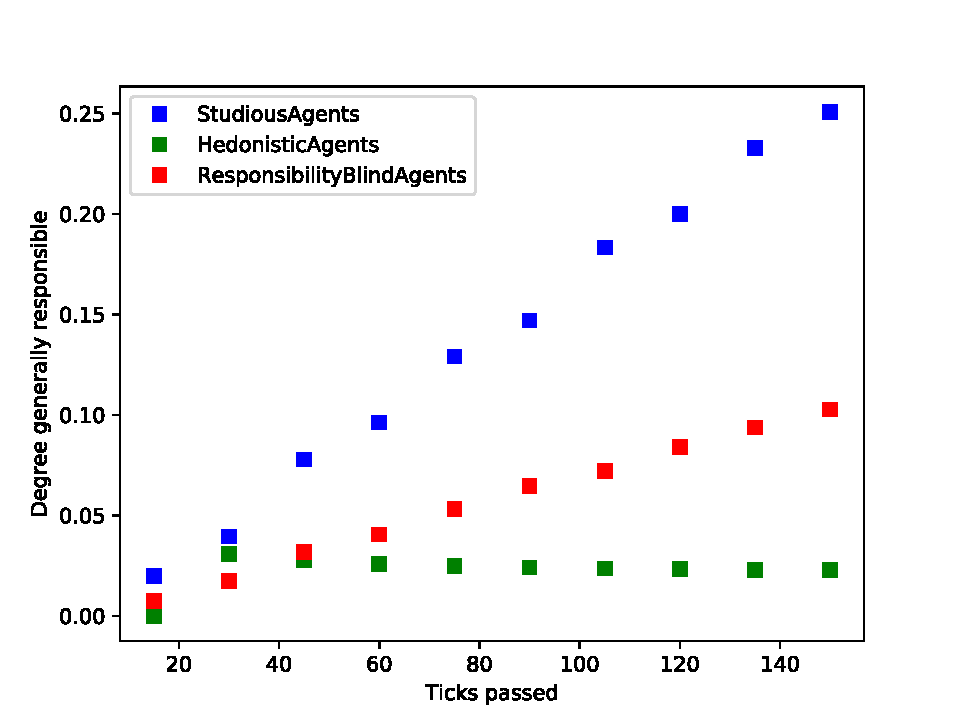
\includegraphics[width=0.5\textwidth]{test_responsibility_directs_behaviour}
    \caption{Agent behaviour over 150 ticks}
    \label{fig:1}
\end{figure}

Responsible agents' behaviours deviate from the ResponsibilityBlindAgents, successfully refuting the null hypothesis. Therefore, the responsibility formalism as outlined \emph{does} direct agent behaviour. The agent behaviour is also directed subjectively, as can be seen in the disparity between StudiousAgents and HedonisticAgents.\par

Notably, while StudiousAgents perform better than ResponsibilityBlindAgents in terms of general measure of responsibility, HedonisticAgents do not. This is an important result: using a responsibility formalism, an agent can perform better than random task selection, making a responsibility a viable task scheduling mechanism which deviates from traditional methods. If improperly calibrated, however, the formalism can perform \emph{worse} than random task selection. This shows that an agent's ability to improve on its performance by directing it's interpretation of responsibility is crucial to real-world applications of the formalism.\par

The predicted plateau of the HedonisticAgents' behaviour is also seen after roughly 30 ticks elapse. This indicates that the interpreting coefficients caused these agents to idle, no longer completing additional tasks, as expected.\par

Research question 1 is answered positively, as a result of the divergent behaviour of all three agent types. Research question 2 should now by explored, as agent behaviour is affirmatively directed by the formalism, but improvements in performance as interpreting coefficients change is yet to be seen.\par

\subsection{RQ 2: Judgement of Responsibility}\label{subsec:RQ2}
A requirement of exploring the second research question is that the advice mechanism outlined in the formalism's design should be utilised. An experiment was therefore devised where HedonisticAgents were advised by a lecturer to adjust interpreting coefficients to resemble those of a StudiousAgent. Advice was given after 100 ticks had elapsed. The resulting simulation can be seen as graphed in \cref{fig:2} with specific responsibility judgement for all agents regarding the resource ``essays\_written'', and in \cref{fig:3} with general responsibility judgement.

\begin{figure}[h]
    \centering
    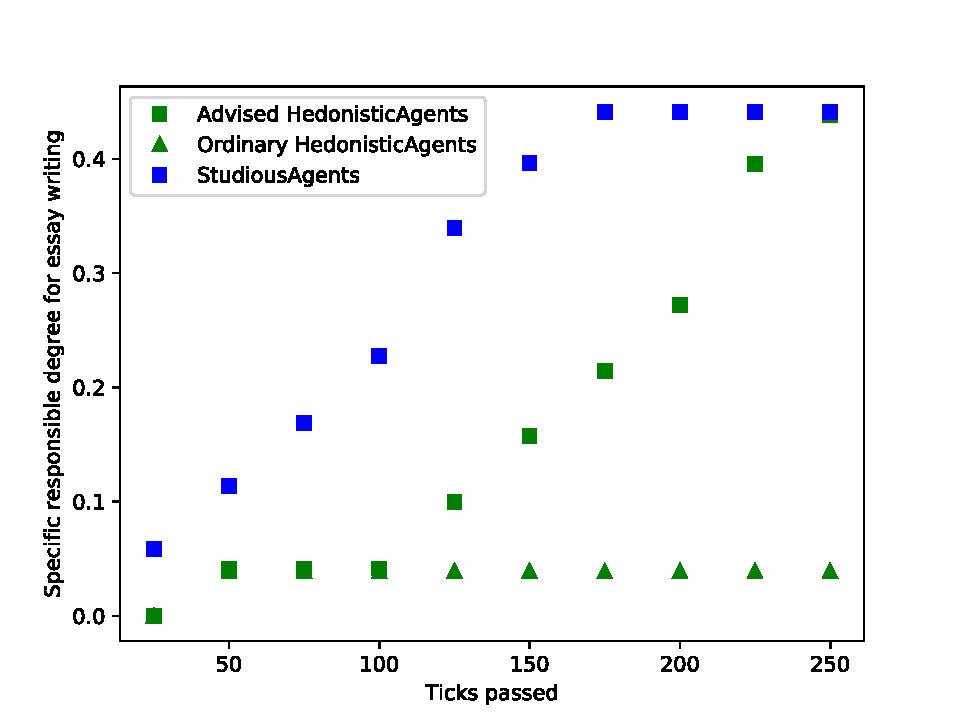
\includegraphics[width=0.5\textwidth]{test_advised_hedonistic_vs_regular_studious251_specific}
    \caption{Specific judgement of ``essays\_written'' responsibility comparing HedonisticAgents with and without advice}
    \label{fig:2}
\end{figure}

\begin{figure}[h]
    \centering
    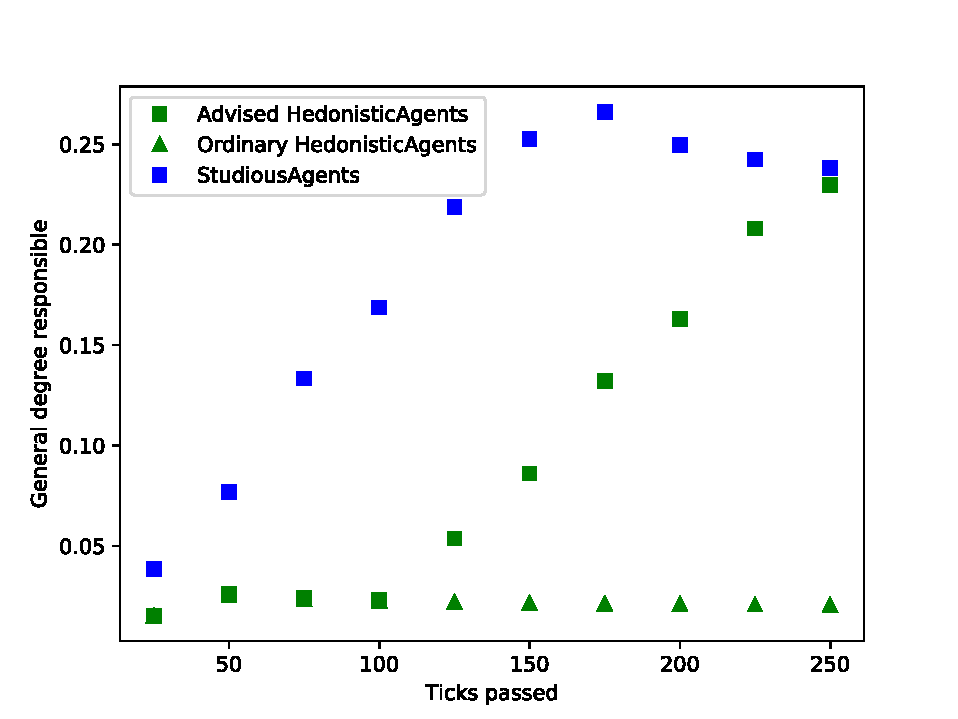
\includegraphics[width=0.5\textwidth]{test_advised_hedonistic_vs_regular_studious251_general}
    \caption{General judgement of responsibility comparing HedonisticAgents with and without advice}
    \label{fig:3}
\end{figure}

As can be seen, immediately after accepting advice, HedonisticAgents deviated from their ordinary behaviour and behaved as StudiousAgents were roughly 100 ticks prior. This pattern is seen in both \cref{fig:2} and \cref{fig:3}, meaning that the advice successfully affected both general and specific responsibility measurements. The outcome of the experiment therefore answers the second research question affirmatively: via the advice functionality, a responsible agent's behaviour can be updated.\par

It is important to note, however, that agents were not providing their own advice. Agents were being identified as performing poorly (as they were HedonisticAgents), asserting that their performance was flawed in some way, and then providing a solution to this flaw in the form of advice. Two problems must yet be solved for agents to supply their own advice:

\begin{enumerate}
    \item Agents must be able to identify their own poor behaviour.\\
        As poor behaviour is identified with interpreted importance scores, an agent will always ``believe'' that it selected optimal responsibilities for discharge. Soliciting advice from respected other agents, or reinterpreting importance scores with the coefficients of respected other agents, is necessary for the proper assessment of poor performance.
    \item Agents must be able to identify corrective measures themselves.\\
        Identifying improper behaviour is a separate task to identifying how to make that behaviour better. Unfortunately, the numbers produced by responsibility judgement do not provide adequate information for identifying corrective behaviour; therefore, additional mechanisms for judgement must be constructed.
\end{enumerate}

The second research question was therefore answered affirmatively, but solving these two additional problems is required for agents to correct their own behaviour independently. While the first problem can be solved with relatively trivial alterations to the presented formalism, the second problem stands as a research question in its own right.\par

\section{Future Work}

\subsection{Independent Behaviour Direction}
The two problems outlined as a requirement to full behaviour direction at the end of \cref{subsec:RQ2} must be solved for the complete independent direction of an agent's behaviour. The first outlined problem is technically solved with a minor modification to the existing formalism; however, the second stands as its own separate research question.\par

In order to solve the second question, an agent may be required to adopt subsets of another agent's interpreting coefficients, or to judge responsibleness in a more nuanced and informative way. One way to assess alternative decisions, and to update interpreting coefficients, would be to build an alternative stack trace of choices another agent would have made, given the same consequential responsibilities. Two potential issues arise with this method, however:

\begin{itemize}
    \item If the other agent had accepted advice in the past, this would need to be taken into account when building a stack trace. Currently, no history of advice taken is kept, making the stack of alternative decisions impossible to properly produce.\par
    \item A history of other responsibilities present when an agent chose to discharge each item in that agent's consequential responsibilities is not kept. This history would be vital to keep, in case delegation revoking were included in a later version of the formalism, or more in-depth analysis on the choice made was required.\par
\end{itemize}

\subsection{Repeated Acts to Discharge a Responsibility}
Currently, an action cannot be repeated multiple times to discharge a Responsibility; instead, a responsibility is discharged only if an act is available with a perfectly matching expected effect.\par

Similarly, some acts may discharge a responsibility with additional side-effects. These do technically fulfil a responsibility's requirements, and should be included also in an ideal formalism.\par

\subsection{Applying The Formalism}
The formalism has been shown to have potential in task scheduling applications. Further work on the formalism, developing enhanced versions with design philosophies more appropriate for specific applications, would prove the real-world and industrial applicability of this research.\par

The formalism at present may be suitable for real-world application for task scheduling. Empirical evidence of this, and any modifications to improve the formalism's performance in more constrained scenarios, will require further research, posing new research questions.\par

\subsection{Integration With Trust}
Similarities between trust and responsibility as social traits were laid out in the background research section of this report. A wealth of insights from trust formalism, including the basic parameters required to construct the formalism presented, were incorporated into the final product.\par

Due to these similarities, and the employment of similar design philosophies between the formalism presented and existing trust formalisms, such as C\&F and Marsh's respective formalisms, development of a model which incorporates the two appears feasible. Each trait's measurements might be used to inform the other in a dual-trait anthropomorphic algorithm, creating a feedback mechanism which allowed each trait to be calculated by a better-informed agent. Dual-trait formalisms usually exist in a format similar to Eigentrust's employment of reputation as a bootstrapping trait for trust; this proposed dual-trait model would instead present two separate traits, measured in parallel, but informing each other.\par

\section{Discussion}
In this report,\todo{paper? dissertation? project?} a new formalism of computational responsibility was presented which is able to direct agent behaviour in a subjective way toward discharging the most important responsibilities earliest.\par

This formalism employs a wealth of insights from sociotechnical literature, as well as literature on trust modelling, the trait with the largest body of anthropomorphic algorithms to date. In this report, the distinction of anthropomorphic algorithms from the rest of sociotechnical literature is defined, as well as its distinction from  human-like computing --- research areas which both affect this smaller field.\par

The presented formalism, applied to a simple sociotechnical modelling scenario, effectively shows that responsibility as it is presented can direct agent behaviour, and is sufficient for significant behavioural changes. It is also shown to perform better than random task selection, where responsible behaviour is required. Improvements to agent behaviour are also demonstrated, ensuring that under-performing agents can become more performant over time by employing the formalism's advice functionality.\par

The formalism successfully answers the research questions --- and answers both affirmatively --- however, it demonstrates the need for further research focus on the trait of responsibility. Presented is a proof-of-concept that responsibility is a valuable trait in anthropomorphic algorithms research; its ultimate application and broader utility can be uncovered only by further work.

\bibliographystyle{abbrv}
\bibliography{biblio}

\end{document}